\documentclass[aspectratio=169]{beamer}

\usetheme{tugraz2018}
\usepackage[english]{babel}


\usepackage{multicol} % for the timetable in the last example only

% two examples for logo-bars (few/many logos):
\newcommand{\myshortexamplelogobar}{Supported by:\qquad
    
\includegraphics[height=.5cm]{figures/logobarexample}\qquad
    
\includegraphics[height=.5cm]{figures/logobarexample}\qquad
    
\includegraphics[height=.5cm]{figures/logobarexample}%
}
\newcommand{\mylongexamplelogobar}{Supported by:\hfill\hfill
    
\includegraphics[height=.5cm]{figures/logobarexample}\hfill
    
\includegraphics[height=.5cm]{figures/logobarexample}\hfill
    
\includegraphics[height=.5cm]{figures/logobarexample}\hfill
    
\includegraphics[height=.5cm]{figures/logobarexample}\hfill
    
\includegraphics[height=.5cm]{figures/logobarexample}%
}

%%%%%%%%%%%%%%%%%%%%%%%%%%%%%%%%%%%%%%%%%%%%%%%%%%%%%%%%%%%%%%%%%%%%%%%%%%%%

\begin{document}

%%%%%%%%%%%%%%%%%%%%%%%%%%%%%%%%%%%%%%%%%%%%%%%%%%%%%%%%%%%%%%%%%%%%%%%%%%%%%%%%

% TITLE
\begin{frame}[plain]
  \subtitle{Examples: POI without Newsline}
  \bottext{For temporary slideshows on digital signage widescreens (POI) during an event}
  \makepoinonewsline
\end{frame}

%%%%%%%%%%%%%%%%%%%%%%%%%%%%%%%%%%%%%%%%%%%%%%%%%%%%%%%%%%%%%%%%%%%%%%%%%%%%%%%%

% EXAMPLE 1: default (gradient gray background, text on top and bottom)
\begin{frame}[plain]
  % define page content
  \subtitle{Untertitel / Subtitle}
  \toptext{POI-Folie mit Text oben\\über vier Zeilen /\\POI Slide with up to\\four lines of text on top}
  \bottext{
    Datum / Date\\
    Ort / Location\\
    > www.tugraz.at/eventwebsite
  }

  % draw page
  \makepoinonewsline
\end{frame}

%%%%%%%%%%%%%%%%%%%%%%%%%%%%%%%%%%%%%%%%%%%%%%%%%%%%%%%%%%%%%%%%%%%%%%%%%%%%%%%%

% EXAMPLE 2: large 'Welcome' text on top, logo on the bottom
\begin{frame}[plain]
  % define page content
  \subtitle{Name der Veranstaltung / Event Name}
  \toptext{\maxsize Herzlich\\willkommen!}
  \bottext{Datum / Date\\
           Ort / Location
  }
  \logobar{\mylongexamplelogobar}

  % draw page
  \makepoinonewsline

  % place additional logos, markers, etc.
  \begin{tikzpicture}[tugtheme]
    % event logo:
    \draw (bottextNE) node[below left] {
\includegraphics[width=3.0cm]{figures/logoexample1}};
  \end{tikzpicture}
\end{frame}

%%%%%%%%%%%%%%%%%%%%%%%%%%%%%%%%%%%%%%%%%%%%%%%%%%%%%%%%%%%%%%%%%%%%%%%%%%%%%%%%

% EXAMPLE 3: blue variant with white text and logo
\begin{frame}[plain]
  % select page style
  \setbeamertemplate{poi page top}[fill] % fill top half with solid color (default: dark blue)
  \setbeamercolor{tuglogo}{fg=white}     % tu graz logo: white text
  \colorlet{main}{titleblue}             % center bar: medium blue

  % define page content
  \toptext{\maxsize Welcome!}
  \subtitle{Name der Veranstaltung / Event Name}
  \bottext{\footnotesize
    Datum / Date\\
    Ort / Location, etc.\\
    www.website.at}
  \logobar{\mylongexamplelogobar}

  % draw page
  \makepoinonewsline

  % place additional logos, markers, etc.
  \begin{tikzpicture}[tugtheme]
    \draw (toptextSE) node[above left] {
\includegraphics[width=6.0cm]{figures/logoexample1}};
  \end{tikzpicture}
\end{frame}

%%%%%%%%%%%%%%%%%%%%%%%%%%%%%%%%%%%%%%%%%%%%%%%%%%%%%%%%%%%%%%%%%%%%%%%%%%%%%%%%

% EXAMPLE 4: default (gradient gray) with an event logo at the top left
\begin{frame}[plain]
  \subtitle{Herzlich willkommen / Welcome!}
  \bottext{Name der Veranstaltung / Event Name\\[4pt]
    \footnotesize
    Datum / Date, Ort / Location, etc.\\
    > www.tugraz.at/go/registration
  }
  \logobar{\mylongexamplelogobar}

  \makepoinonewsline

  \begin{tikzpicture}[tugtheme]
    % event logo:
    \draw (toptextSW) node[above right] {
\includegraphics[width=8.5cm]{figures/logoexample1}};
  \end{tikzpicture}
\end{frame}

%%%%%%%%%%%%%%%%%%%%%%%%%%%%%%%%%%%%%%%%%%%%%%%%%%%%%%%%%%%%%%%%%%%%%%%%%%%%%%%%

% EXAMPLE 5: with photo on the top right and text on top
\begin{frame}[plain]
  \colorlet{main}{titleblue}

  \subtitle{Willkommen / Welcome!}
  \bottext{\footnotesize
    Veranstaltungsname / Event name\\
    Datum / Date \\
    Ort / Location, etc.}
  \logobar{\mylongexamplelogobar}

  \makepoinonewsline

  \begin{tikzpicture}[tugtheme]
    % event logo:
    \draw (toptextSW) node[above right] {
\includegraphics[width=7.0cm]{figures/logoexample1}};
    % custom (flipped) image and copyright information:
    \draw (toprightlogoSE) node[anchor=south west,xscale=-1] {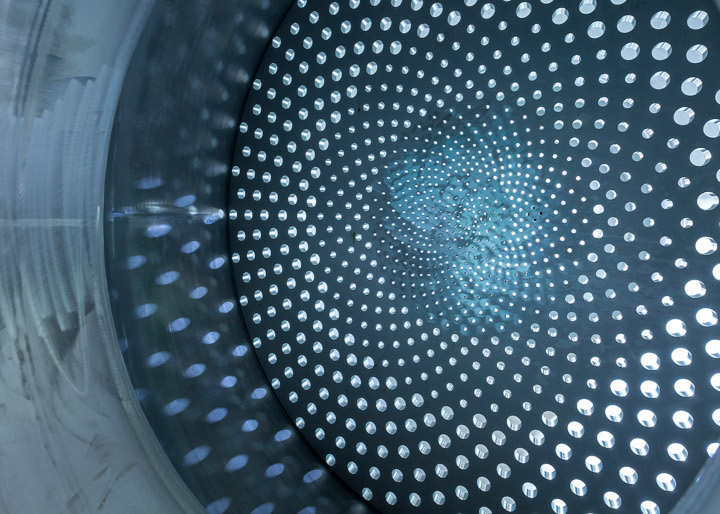
\includegraphics[width=6.75cm]{figures/photoexample-43}}
                           node[above left, copyright] {\copyright\ Lunghammer -- TU Graz};
  \end{tikzpicture}
\end{frame}

%%%%%%%%%%%%%%%%%%%%%%%%%%%%%%%%%%%%%%%%%%%%%%%%%%%%%%%%%%%%%%%%%%%%%%%%%%%%%%%%

% EXAMPLE 6: with photo on the top right and logo on top
\begin{frame}[plain]
  \toptext{\huge Name der\\Veranstaltung /\\Event Name}
  \subtitle{Willkommen / Welcome!}
  \bottext{\footnotesize
    Zusatztext mit Textlänge für zwei Zeilen / \\
    Additional description of up to two lines\\
    Datum / Date, Ort / Location, etc.}
  \logobar{\mylongexamplelogobar}

  \makepoinonewsline

  \begin{tikzpicture}[tugtheme]
    % event logo:
    \draw (bottextNE) node[below left] {
\includegraphics[width=3.5cm]{figures/logoexample1}};
    % custom (flipped) image and copyright information:
    \draw (toprightlogoSE) node[anchor=south west,xscale=-1] {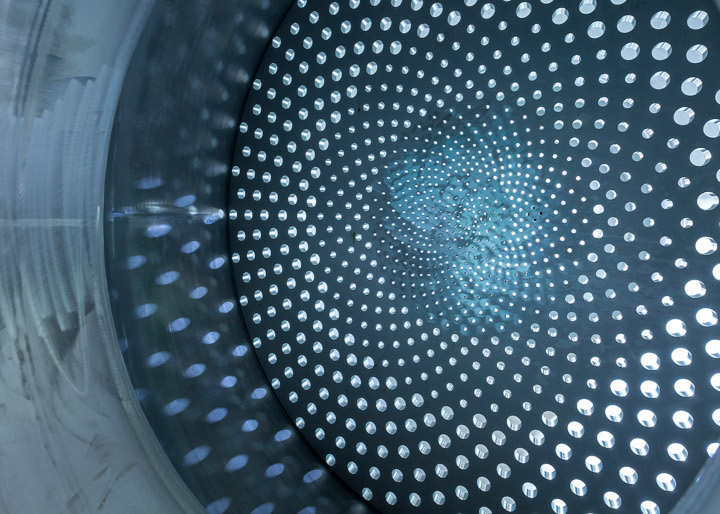
\includegraphics[width=6.75cm]{figures/photoexample-43}}
                           node[above left, copyright] {\copyright\ Lunghammer -- TU Graz};
  \end{tikzpicture}
\end{frame}

%%%%%%%%%%%%%%%%%%%%%%%%%%%%%%%%%%%%%%%%%%%%%%%%%%%%%%%%%%%%%%%%%%%%%%%%%%%%%%%%

% EXAMPLE 7: with photo (Alte Technik) on top
\begin{frame}[plain]
  \setbeamercolor{tuglogo}{fg=white}
  \titlefigure{figures/topfigureexample-169-poi-nonewsline}

  \subtitle{Herzlich willkommen!}
  \bottext{%
    Name der Veranstaltung /\\
    Event Name\\
    \footnotesize
    Datum / Date\\
    Ort / Location, etc.
  }

  \makepoinonewsline

  \begin{tikzpicture}[tugtheme]
    % event logo (bottom right):
    \draw (bottextSE) node[above left] {
\includegraphics[width=3.5cm]{figures/logoexample1}};
    % image copyright:
    \draw (topcopyrightSE) node[above left, copyright] {\copyright\ Lunghammer -- TU Graz};
  \end{tikzpicture}
\end{frame}

%%%%%%%%%%%%%%%%%%%%%%%%%%%%%%%%%%%%%%%%%%%%%%%%%%%%%%%%%%%%%%%%%%%%%%%%%%%%%%%%

% EXAMPLE 8: with photos (montage) on top
\begin{frame}[plain]
  \titlefigure{figures/topfigureexample-montage2-169-poi}
  \colorlet{main}{titleblue}

  \subtitle{Name der Veranstaltung / Event Name}
  \bottext{\footnotesize
    Zusatztext mit Textlänge für zwei Zeilen / \\
    Additional description of up to two lines\\
    Datum / Date\\
    Ort / Location, etc.}
  \logobar{\myshortexamplelogobar}

  \makepoinonewsline

  \begin{tikzpicture}[tugtheme]
    \draw (bottextSE) node[above left] {
\includegraphics[width=3.5cm]{figures/logoexample2}};
    \draw (topcopyrightSE) node[above left, copyright] {\copyright\ Lunghammer -- TU Graz};
  \end{tikzpicture}
\end{frame}

%%%%%%%%%%%%%%%%%%%%%%%%%%%%%%%%%%%%%%%%%%%%%%%%%%%%%%%%%%%%%%%%%%%%%%%%%%%%%%%%

% EXAMPLE 9: with background photo and text on top
\begin{frame}[plain]
  \titlefigure{figures/topfigureexample-detail-169-poi-nonewsline}
  %\setbeamercolor{welcome page top}{fg=white} % change top font color if necessary
  \setbeamercolor{tuglogo}{fg=white}
  \colorlet{main}{titleblue}

  \toptext{%
    Titel / Title\\
    \large
    Name der Veranstaltung /\\
    Event name}
  \subtitle{Herzlich willkommen / Welcome!}
  \bottext{\footnotesize
    Datum / Date \\
    Ort / Location, etc.\\
    > www.website.at}
  \logobar{\myshortexamplelogobar}

  \makepoinonewsline

  \begin{tikzpicture}[tugtheme]
    \draw (bottextSE) node[above left] {
\includegraphics[width=3.5cm]{figures/logoexample2}};
    \draw (topcopyrightSE) node[above left, copyright] {\copyright\ Lunghammer -- TU Graz};
  \end{tikzpicture}
\end{frame}

%%%%%%%%%%%%%%%%%%%%%%%%%%%%%%%%%%%%%%%%%%%%%%%%%%%%%%%%%%%%%%%%%%%%%%%%%%%%%%%%

% EXAMPLE 10: with event program (one column) on dark background on top
\begin{frame}[plain]
  \setbeamertemplate{poi page top}[fill]
  \setbeamercolor{tuglogo}{fg=white}
  \colorlet{main}{titleblue}

  \toptext{
    \begin{tugtimetable}
      \item[19:30 Uhr]
        \textbf{Das ist ein sehr langer Titel des Vortrags und\\er enthält Text über mehrere Zeilen}\\
        Vorname Nachname\\
        Institution / Unternehmen
      \item[20:15 Uhr]
        \textbf{Das ist ein sehr langer Titel des Vortrags und\\er enthält Text über mehrere Zeilen}\\
        Vorname Nachname\\
        Institution / Unternehmen
    \end{tugtimetable}
  }
  \subtitle{Name der Veranstaltung / Event name}
  \bottext{\footnotesize
    Datum / Date \\
    Ort / Location, etc.\\
    > www.website.at}
  \logobar{\myshortexamplelogobar}

  \makepoinonewsline

  \begin{tikzpicture}[tugtheme]
    \draw (bottextSE) node[above left] {
\includegraphics[width=3.5cm]{figures/logoexample2}};
  \end{tikzpicture}
\end{frame}

%%%%%%%%%%%%%%%%%%%%%%%%%%%%%%%%%%%%%%%%%%%%%%%%%%%%%%%%%%%%%%%%%%%%%%%%%%%%%%%%

% EXAMPLE 11: with event program (two columns) on standard gradient gray background on top
\begin{frame}[plain]
  %\setbeamertemplate{poi page top}[plain]  % select white top background
  \toptext{
    \begin{tugtimetabletwocolumn}
      \item[12:00] Programmpunkt 1
      \item[12:30] Programmpunkt 2
      \item[13:30] Programmpunkt 3
      \item[14:30] Programmpunkt 4
      \item[15:30] Programmpunkt 5\\
                   ganz unten
      \item[17:00] Titel eines Vortrags\\
                   Vorname Nachname\\
                   Institution
      \item[18:00] Programmpunkt 7
      \item[19:00] Programmpunkt 8\\
                   mit zwei Zeilen
      \item[20:00] Programmpunkt 9\\
                   mit zwei Zeilen
    \end{tugtimetabletwocolumn}
  }
  \subtitle{PROGRAMM 12:00--20:00 Uhr}
  \bottext{Name der Veranstaltung /\\
    Event Name\\
    \footnotesize
    Datum / Date \\
    Ort / Location, etc.}

  \makepoinonewsline

  \begin{tikzpicture}[tugtheme]
    \draw (bottextSE) node[above left] {
\includegraphics[width=3.5cm]{figures/logoexample1}};
  \end{tikzpicture}
\end{frame}

%%%%%%%%%%%%%%%%%%%%%%%%%%%%%%%%%%%%%%%%%%%%%%%%%%%%%%%%%%%%%%%%%%%%%%%%%%%%%%%%

% AVAILABLE TikZ COORDINATES
\begin{frame}[plain]
  \subtitle{Available Coordinates}
  \title{}
  \bottext{\bigskip Rectangle corners: \texttt{NW} (labelled, e.g., \texttt{topNW}), \texttt{SW}, \texttt{NE}, \texttt{SE}}
  \makepoinonewsline

  \begin{tikzpicture}[tugtheme,font=\ttfamily\small,thick]
    \draw (topNW) node[below right] {top} rectangle (topSE);
    \draw (toptextNW) node[below right] {toptext/toptextalt} rectangle (toptextSE)
          (toptextNW) rectangle (toptextaltSE);
    \draw (barNW) node[below right] {bar} rectangle (barSE);
    \draw (bartextNW) node[below right] {bartext} rectangle (bartextSE);
    \draw (botNW) node[below right] {bot} rectangle (botSE);
    \draw (footNW) node[below right] {foot} rectangle (footSE);
    \draw (bottextNW) node[below right] {bottext/bottextalt} rectangle (bottextSE)
          (bottextNW) rectangle (bottextaltSE);
    \draw (toprightlogoSE) node[fill,circle,minimum size=3pt] {} node[above left] {toprightlogoSE};
    \draw (topcopyrightSE) node[fill,circle,minimum size=3pt] {} node[above left] {topcopyrightSE};

  \end{tikzpicture}
\end{frame}

\end{document}
